% !TEX program = xelatex
\documentclass[12pt,a4paper]{ctexart}
\usepackage[top=2.25cm,bottom=2.25cm,left=2.35cm,right=2.35cm,headheight=15pt]{geometry}
\usepackage{amsmath,amssymb,booktabs,array,longtable,multirow}
\usepackage{graphicx,float,caption,subcaption}
\usepackage{xcolor,enumitem,fancyhdr,hyperref,titlesec}
\usepackage[most]{tcolorbox}
\usepackage{tikz}
\usetikzlibrary{arrows.meta,positioning,fit}
\graphicspath{{../output/charts/}}
% 此文件由 main.py 自动生成，不要手工修改。
\newcommand{\ModelAUC}{0.856}
\newcommand{\ModelPRAUC}{0.734}
\newcommand{\ModelBrier}{0.107}
\newcommand{\ModelLogLoss}{0.357}
\newcommand{\ModelLTwo}{0.10}
\newcommand{\ModelFeatureCount}{16}
\newcommand{\AttachmentOneEnterprises}{123}
\newcommand{\AttachmentTwoEnterprises}{302}
\newcommand{\AttachmentOneInvoices}{373431}
\newcommand{\AttachmentTwoInvoices}{726010}
\newcommand{\KnownDefaults}{27}
\newcommand{\KnownDefaultRate}{22.0}
\newcommand{\PoneLoanCount}{80}
\newcommand{\PtwoLoanCount}{100}
\newcommand{\PthreeLoanCount}{100}
\newcommand{\PoneAmount}{8000}
\newcommand{\PtwoAmount}{10000}
\newcommand{\PthreeAmount}{10000}
\newcommand{\PoneAverageRate}{12.31}
\newcommand{\PtwoAverageRate}{10.28}
\newcommand{\PthreeAverageRate}{10.35}
\newcommand{\PoneNetProfit}{70.54}
\newcommand{\PtwoNetProfit}{133.56}
\newcommand{\PthreeNetProfit}{132.19}
\newcommand{\EmergencyChanges}{8}
\newcommand{\SensitivityMean}{0.9983}
\newcommand{\SensitivityMin}{0.9958}
\newcommand{\SensitivityKendall}{0.9729}
\newcommand{\SensitivityIndicator}{年化利润}
\newcommand{\SensitivityRemoval}{0.9150}
\newcommand{\OriginalDLoanCount}{0}
\newcommand{\GradeACount}{56}
\newcommand{\GradeADefaults}{3}
\newcommand{\GradeARate}{5.4}
\newcommand{\GradeAPD}{5.6}
\newcommand{\GradeBCount}{32}
\newcommand{\GradeBDefaults}{4}
\newcommand{\GradeBRate}{12.5}
\newcommand{\GradeBPD}{13.6}
\newcommand{\GradeCCount}{15}
\newcommand{\GradeCDefaults}{4}
\newcommand{\GradeCRate}{26.7}
\newcommand{\GradeCPD}{28.8}
\newcommand{\GradeDCount}{20}
\newcommand{\GradeDDefaults}{16}
\newcommand{\GradeDRate}{80.0}
\newcommand{\GradeDPD}{61.1}


\definecolor{navy}{HTML}{17324D}
\definecolor{teal}{HTML}{0F766E}
\definecolor{pale}{HTML}{EDF5F4}
\definecolor{linegray}{HTML}{D9E2E7}
\hypersetup{colorlinks=true,linkcolor=navy,urlcolor=teal,citecolor=teal}
\setlength{\parindent}{2em}
\setlength{\parskip}{3pt}
\setlist{nosep,leftmargin=2em}
\pagestyle{fancy}
\fancyhf{}
\fancyhead[C]{中小微企业的信贷决策研究}
\fancyfoot[C]{\thepage}
\renewcommand{\headrulewidth}{0.4pt}
\titleformat{\section}{\Large\bfseries\color{navy}}{\thesection}{0.8em}{}
\titleformat{\subsection}{\large\bfseries}{\thesubsection}{0.7em}{}
\captionsetup{font=small,labelsep=quad}

\newtcolorbox{intuitionbox}[1]{
  colback=pale,colframe=teal,boxrule=0.7pt,arc=2mm,
  left=8pt,right=8pt,top=6pt,bottom=6pt,
  title={直觉理解：#1},fonttitle=\bfseries,coltitle=navy
}
\newtcolorbox{decisionbox}[1]{
  colback=white,colframe=navy,boxrule=0.7pt,arc=2mm,
  left=8pt,right=8pt,top=6pt,bottom=6pt,
  title={银行视角：#1},fonttitle=\bfseries,coltitle=navy
}

\title{\vspace{-1.7cm}\heiti\zihao{2}中小微企业的信贷决策研究\\
\vspace{0.3cm}\normalfont\zihao{4}基于监督违约概率、单调流失率与混合整数规划}
\author{\zihao{4}冯浩然}
\date{}

\begin{document}
\maketitle

\begin{center}
\begin{minipage}{0.94\textwidth}
\zihao{-5}
\textbf{摘要：}
针对仅有企业基础信息和进销项发票、且有标签样本仅\AttachmentOneEnterprises 家的中小微企业信贷决策问题，本文建立“监督违约概率、经营质量辅助解释、利率与额度联合优化、突发冲击重优化”的闭环模型。首先保留有效发票金额的正负符号，按连续自然月补零，构造规模、盈利、稳定性、活跃度、趋势、作废及红冲等\ModelFeatureCount 个特征。随后采用带$L_2$正则和类别平衡权重的逻辑回归估计违约概率，通过5次重复的5折嵌套分层交叉验证获得严格样本外预测，并用固定PD阈值划分A至D四档。模型样本外ROC-AUC为\ModelAUC，PR-AUC为\ModelPRAUC，Brier分数为\ModelBrier。TOPSIS不再承担违约预测，而是在附件1确定缩放边界和理想点后迁移至附件2，用于解释经营质量。对附件3采用保序回归得到随利率非降的客户流失率曲线，并以留存后利息、违约损失和资金成本构造单位额度期望收益。在原始D级和预测D级禁贷、单户额度为0或10至100万元、总预算精确满足的条件下，用混合整数线性规划配置贷款。疫情冲击通过赔率乘数作用于PD后重新评级、定价和分配。最终问题1、2、3分别向\PoneLoanCount、\PtwoLoanCount、\PthreeLoanCount 家企业授信，期望净收益分别为\PoneNetProfit、\PtwoNetProfit、\PthreeNetProfit 万元。100次真实权重扰动的Spearman相关系数均值为\SensitivityMean。模型把预测、定价、分配和压力测试放入同一可复算流程，并明确区分数据事实、模型结果和业务假设。

\textbf{关键词：}中小微企业；违约概率；逻辑回归；保序回归；混合整数规划；信贷定价
\end{minipage}
\end{center}

\newpage
\tableofcontents
\newpage

\section{问题重述与任务拆解}

某银行拟向中小微企业发放一年期贷款，单户额度为10至100万元，年利率范围为4\%至15\%。附件1给出\AttachmentOneEnterprises 家有信贷记录企业的信誉评级、是否违约标签以及进销项发票；附件2给出\AttachmentTwoEnterprises 家无信贷记录企业的基础信息和发票；附件3给出不同信誉等级下贷款利率与客户流失率的统计关系。

题目表面上要求给出额度和利率，实际包含四个连续问题：

\begin{enumerate}
\item 如何把几十万张发票压缩为能够反映经营状况的企业特征；
\item 如何用有标签企业学习“未来发生违约的可能性”；
\item 如何在利率收入、客户流失、违约损失和资金成本之间取舍；
\item 如何在预算、禁贷和单户上下限约束下形成可执行的组合方案。
\end{enumerate}

如果只给企业排一个综合名次，就无法回答“违约概率是多少”；如果只预测违约概率，又无法回答“利率和额度是多少”。因此本文把问题拆成风险预测、经营解释、定价和组合优化四层，每层只承担一个明确任务。

\begin{intuitionbox}{把整道题看成银行的一条决策流水线}
发票数据回答企业过去经营得怎么样；监督模型回答企业未来违约的可能性；流失率模型回答客户是否愿意接受某个利率；优化模型回答有限资金应当投给谁。前一层的输出是后一层的输入，而不是四个互不相关的方法。
\end{intuitionbox}

\section{问题分析与总体建模路线}

\subsection{为什么不能直接使用银行原评级}

附件2没有银行信誉评级，原评级无法直接迁移；同时，附件1的评级是人工综合判断，不等同于真实违约标签。本文保留原评级用于准入约束和对照分析，但用“是否违约”训练概率模型。这样既尊重银行已有规则，也使附件2获得统一的风险尺度。

\subsection{为什么TOPSIS不是风险主模型}

TOPSIS适合回答“哪个企业更接近理想经营状态”，但它没有直接利用违约标签。若把TOPSIS分数直接当作PD，会把经营质量排序和违约概率混为一谈。因此本文用逻辑回归估计PD，用TOPSIS解释企业经营质量，二者职责分开。

\subsection{完整流程}

\begin{figure}[H]
\centering
\begin{tikzpicture}[
node distance=7mm and 5mm,
box/.style={draw=navy,rounded corners=2mm,minimum width=2.75cm,minimum height=1.0cm,align=center,fill=white},
sub/.style={draw=teal,rounded corners=2mm,minimum width=2.75cm,minimum height=1.0cm,align=center,fill=pale},
arr/.style={-{Latex[length=2mm]},thick,color=navy}
]
\node[box] (raw) {原始企业信息\\进销项发票};
\node[box,right=of raw] (feat) {净额与连续月历\\16项PD特征};
\node[box,right=of feat] (pd) {监督逻辑回归\\样本外PD};
\node[box,right=of pd] (grade) {固定PD档位\\A、B、C、D};
\node[box,below=of grade] (profit) {保序流失率与收益\\最优利率};
\node[box,left=of profit] (milp) {MILP额度分配\\预算与准入约束};
\node[box,left=of milp] (shock) {疫情赔率冲击\\重新评级与优化};
\node[sub,left=of shock] (topsis) {固定尺度TOPSIS\\经营质量解释支线};
\draw[arr] (raw) -- (feat);
\draw[arr] (feat) -- (pd);
\draw[arr] (pd) -- (grade);
\draw[arr] (grade) -- (profit);
\draw[arr] (profit) -- (milp);
\draw[arr] (milp) -- (shock);
\draw[-{Latex[length=2mm]},thick,dashed,color=teal]
  (feat.south) -- ++(0,-3mm) -| (topsis.north);
\end{tikzpicture}
\caption{从原始发票到信贷策略的完整流程}
\end{figure}

\begin{decisionbox}{流程图如何阅读}
PD是风险主线，TOPSIS是解释支线。流失率把利率和客户接受行为连接起来，MILP把单户最优收益转化为全行预算下的组合方案。疫情发生后不是简单缩减原额度，而是重新运行PD调整、评级、定价和额度优化。
\end{decisionbox}

\section{数据理解、基本假设与符号}

\subsection{数据规模}

附件1共有\AttachmentOneInvoices 条进销项发票，附件2共有\AttachmentTwoInvoices 条。附件1中已知违约企业为\KnownDefaults 家，样本违约率为\KnownDefaultRate\%。附件3包含29个利率与流失率观测点。数据量最大的部分是票据明细，而真正用于监督学习的企业样本只有123家，因此模型应优先稳定和可解释，不宜盲目使用复杂黑箱。

\begin{figure}[H]
\centering
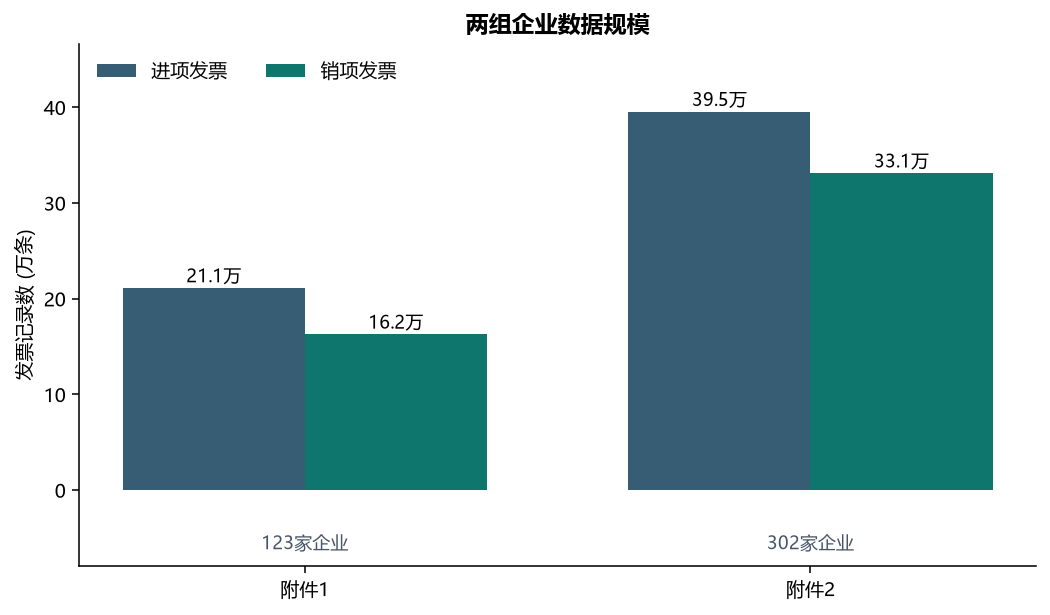
\includegraphics[width=0.78\textwidth]{fig_data_scale.png}
\caption{附件1与附件2的数据规模}
\end{figure}

\subsection{基本假设}

\begin{table}[H]
\centering
\caption{主要假设及其作用}
\small
\begin{tabular}{p{3.1cm}p{2.2cm}p{8.0cm}}
\toprule
假设 & 取值 & 说明\\
\midrule
贷款期限 & 1年 & 与题目一致，利率和损失均按一年期计算\\
问题1预算 & 8000万元 & 题目未明确给出，作为可配置情景，不把它视为数据事实\\
问题2与3预算 & 10000万元 & 按题目给出的1亿元年度额度\\
违约损失率LGD & 60\% & 违约后本金的期望损失比例，可由银行回收数据替换\\
资金成本率 & 2.5\% & 银行投放资金的机会成本，可按真实资金价格更新\\
客户流失 & 不接受贷款 & 流失客户不产生放款、利息、损失和资金成本\\
行业冲击 & 作用于赔率 & 用于情景压力测试，不视为疫情的精确因果估计\\
\bottomrule
\end{tabular}
\end{table}

\subsection{主要符号}

\begin{longtable}{p{1.7cm}p{4.3cm}p{7.5cm}}
\caption{主要符号说明}\\
\toprule
符号 & 名称 & 含义\\
\midrule
\endfirsthead
\toprule
符号 & 名称 & 含义\\
\midrule
\endhead
$i$ & 企业索引 & 附件中的某一家企业\\
$y_i$ & 违约标签 & 违约取1，不违约取0\\
$\boldsymbol x_i$ & 特征向量 & 企业的规模、盈利、稳定性、活跃度和票据行为\\
$p_i$ & 违约概率PD & 模型预测企业一年内违约的概率\\
$r_i$ & 贷款年利率 & 在附件3的观测利率网格上选择\\
$c_i(r)$ & 客户流失率 & 企业面对利率$r$时拒绝贷款的概率\\
$q_i(r)$ & 客户留存率 & $q_i(r)=1-c_i(r)$\\
$L$ & LGD & 违约时的损失比例，本文取60\%\\
$c_f$ & 资金成本率 & 本文取2.5\%\\
$u_i(r)$ & 单位额度期望收益 & 每投放1万元给企业$i$的期望净收益\\
$x_i$ & 授信额度 & 企业$i$获得的名义贷款额度，单位为万元\\
$z_i$ & 选择变量 & 获贷为1，不获贷为0\\
$B$ & 总预算 & 问题1为8000万元，问题2和3为10000万元\\
$k_i$ & 疫情冲击系数 & 乘到企业的违约赔率上\\
\bottomrule
\end{longtable}

\section{从发票到企业特征}

\subsection{票据口径与有符号净额}

对状态为“有效发票”的记录使用不含税金额列，并保留正负符号。正数票据表示正常交易，负数票据通常对应红冲或退货，应冲减而不是取绝对值。企业$i$的销项净额定义为
\begin{equation}
R_i=\sum_{j\in\mathcal V_i^{out}}a_{ij},
\end{equation}
其中$\mathcal V_i^{out}$为有效销项票据集合，$a_{ij}$为有符号金额。进项净额$C_i$同理。税额不与金额重复相加；作废票据不进入净额，但其数量进入作废率特征。

\begin{intuitionbox}{为什么负数发票不能取绝对值}
假设企业先开出100万元销项发票，随后发生20万元退货并开具$-20$万元红冲票。真实销售净额是$100-20=80$万元。如果对负数取绝对值，就会得到$100+20=120$万元，收入被高估50\%。若20万元票据是作废票，则它完全不进入净额，但会提高作废率。
\end{intuitionbox}

\subsection{连续月历与经营断档}

对每家企业，从第一张到最后一张有效票据构造连续自然月序列，无交易月份补0。设观察月数为$M_i$，有交易的月份为$A_i$，则
\begin{equation}
\mathrm{ActiveRatio}_i=\frac{A_i}{M_i},\qquad
\mathrm{AnnualRevenue}_i=\frac{12R_i}{M_i}.
\end{equation}

\begin{intuitionbox}{补0和删除月份有什么区别}
一家企业6个月内只有1月和6月有收入。如果只保留有收入的两个月，它看起来“每个月都在经营”；补齐2月至5月的0之后，活跃月份比例只有$2/6$，中间断档被保留下来。风险模型由此能够区分持续经营与偶发大额交易。
\end{intuitionbox}

最近断档月数记录最后一个有交易月份至观察期末的间隔；收入和成本波动率使用连续月序列标准差除以平均绝对规模；趋势率由月份序号对月净额的线性斜率再除以平均绝对规模得到。所有分母为0的比率按0处理，最终数值列检查并消除缺失值和无穷值。

\subsection{16项PD特征}

\begin{table}[H]
\centering
\caption{监督PD模型的特征分组}
\small
\begin{tabular}{p{2.4cm}p{5.1cm}p{6.0cm}}
\toprule
维度 & 特征 & 风险含义\\
\midrule
规模与盈利 & 年化销项净额、年化利润、利润率、年化客户数、年化供应商数 & 衡量经营规模、盈利空间和交易网络\\
稳定与趋势 & 收入波动率、成本波动率、收入趋势率 & 识别经营剧烈波动或持续收缩\\
经营连续性 & 活跃月份比例、最近断档月数 & 识别长期停顿和低频经营\\
票据行为 & 进销项作废率、负数发票率、负数金额率 & 反映作废、红冲、退货等异常或经营特征\\
\bottomrule
\end{tabular}
\end{table}

年化销项净额、年化利润、客户数和供应商数呈明显长尾，先做有符号对数变换
\begin{equation}
T(x)=\operatorname{sign}(x)\log(1+|x|),
\end{equation}
再用训练折的1\%和99\%分位点截尾，并按训练折均值、标准差进行标准化。验证折和附件2只应用训练阶段得到的参数，避免把未来或待预测数据的信息泄漏进模型。

\section{监督违约概率模型}

\subsection{为什么选择正则逻辑回归}

附件1只有123家企业和27个违约样本。复杂模型虽然能提高训练集拟合度，却可能只记住少数企业。逻辑回归直接输出0至1之间的概率，系数方向可解释，配合$L_2$正则能抑制小样本下的系数剧烈波动，因此适合作为主模型\cite{hosmer2013,hastie2009}。

令$y_i=1$表示违约，标准化特征向量为$\boldsymbol x_i$，线性风险得分为
\begin{equation}
z_i=\beta_0+\boldsymbol x_i^{\mathsf T}\boldsymbol\beta,
\end{equation}
再通过Sigmoid函数转为PD：
\begin{equation}
\hat p_i=\sigma(z_i)=\frac{1}{1+e^{-z_i}}.
\end{equation}

\begin{intuitionbox}{线性得分如何变成概率}
如果某企业的标准化特征经过系数加权后得到$z=0$，则$\sigma(0)=0.5$；若$z=-2$，PD约为11.9\%；若$z=2$，PD约为88.1\%。Sigmoid函数把任意实数压缩到0和1之间，同时保留风险高低顺序。
\end{intuitionbox}

\subsection{类别平衡与L2正则}

非违约企业明显多于违约企业。如果所有企业权重相同，模型可能偏向多数类。本文让两类样本的总训练权重各占一半：
\begin{equation}
w_i=\begin{cases}
\dfrac{n}{2n_1},&y_i=1,\\[4pt]
\dfrac{n}{2n_0},&y_i=0,
\end{cases}
\end{equation}
其中$n_1,n_0$分别为违约和非违约数量。优化目标为
\begin{equation}
\min_{\beta_0,\boldsymbol\beta}
\frac{1}{\sum_iw_i}\sum_iw_i\left[\log(1+e^{z_i})-y_iz_i\right]
+\frac{\lambda}{2}\|\boldsymbol\beta\|_2^2.
\end{equation}

后一项是$L_2$惩罚。$\lambda$越大，系数越接近0，模型更平滑但可能欠拟合；$\lambda$越小，模型更贴合训练数据但可能过拟合。最终全样本模型选择$\lambda=\ModelLTwo$。

\subsection{为什么还需要先验校正}

类别平衡让训练过程暂时把两类看得同样重要，但真实样本违约率只有\KnownDefaultRate\%。若直接输出平衡训练概率，会系统性高估PD。因此在预测时把训练折真实违约率$\pi$的对数赔率加回：
\begin{equation}
\hat p_i=\sigma\left(\hat z_i+\log\frac{\pi}{1-\pi}\right).
\end{equation}

这一步不改变企业大致风险顺序，但把概率水平拉回真实样本基准。它回答的是“在真实违约率背景下，这家企业大约有多大风险”，而不是“在两类被人为平衡后，模型有多确信”。

\subsection{嵌套重复样本外验证}

若在训练模型的同一批企业上评价，模型可能因为记住样本而显得过于优秀。本文采用外层5次重复、每次5折的分层交叉验证；每个外层训练集内部再用4折交叉验证，从$\{0.01,0.1,1,10\}$中选择$\lambda$。

一次外层循环的步骤是：

\begin{enumerate}
\item 把约80\%企业作为外层训练集，约20\%作为外层测试集，并保持违约比例接近；
\item 只在外层训练集内部选择$\lambda$；
\item 只用外层训练集计算截尾点、均值和标准差；
\item 训练模型并预测从未参与训练的外层测试企业；
\item 重复直到每家企业都获得一次样本外预测；更换随机划分后再重复5次，最后取均值。
\end{enumerate}

\begin{intuitionbox}{内层和外层分别做什么}
内层负责“选模型”，例如决定正则强度；外层负责“考模型”，只评价已经选好的完整流程。如果用同一折既选参数又报成绩，测试集就间接参与了模型选择，结果仍会偏乐观。
\end{intuitionbox}

\section{PD等级与模型验证}

\subsection{固定风险档位}

为使不同附件和未来批次具有相同含义，PD档位采用固定阈值，而不是每批企业按人数分位数强行分组：
\begin{equation}
g(p)=\begin{cases}
A,&0\le p<0.10,\\
B,&0.10\le p<0.20,\\
C,&0.20\le p<0.40,\\
D,&p\ge0.40.
\end{cases}
\end{equation}

\subsection{四个验证指标怎样理解}

\begin{itemize}
\item \textbf{ROC-AUC}：随机抽取一个违约企业和一个非违约企业，模型把违约企业排在更高风险位置的概率。0.5近似随机，越接近1越好。
\item \textbf{PR-AUC}：关注高风险名单中违约企业能否被找出，特别适合违约样本较少的情况。
\item \textbf{Brier分数}：预测概率与0/1真实结果的平均平方差，越小越好。它同时惩罚过高和过低的概率。
\item \textbf{Log Loss}：对“非常自信但判断错误”的预测处罚更重，越小越好。
\end{itemize}

\begin{table}[H]
\centering
\caption{重复嵌套样本外预测性能}
\begin{tabular}{lcccc}
\toprule
指标 & ROC-AUC & PR-AUC & Brier & Log Loss\\
\midrule
数值 & \ModelAUC & \ModelPRAUC & \ModelBrier & \ModelLogLoss\\
\bottomrule
\end{tabular}
\end{table}

\begin{table}[H]
\centering
\caption{固定PD档位的样本外违约表现}
\begin{tabular}{ccccc}
\toprule
等级 & 企业数 & 违约数 & 实际违约率 & 平均预测PD\\
\midrule
A & \GradeACount & \GradeADefaults & \GradeARate\% & \GradeAPD\%\\
B & \GradeBCount & \GradeBDefaults & \GradeBRate\% & \GradeBPD\%\\
C & \GradeCCount & \GradeCDefaults & \GradeCRate\% & \GradeCPD\%\\
D & \GradeDCount & \GradeDDefaults & \GradeDRate\% & \GradeDPD\%\\
\bottomrule
\end{tabular}
\end{table}

\begin{figure}[H]
\centering
\begin{subfigure}{0.49\textwidth}
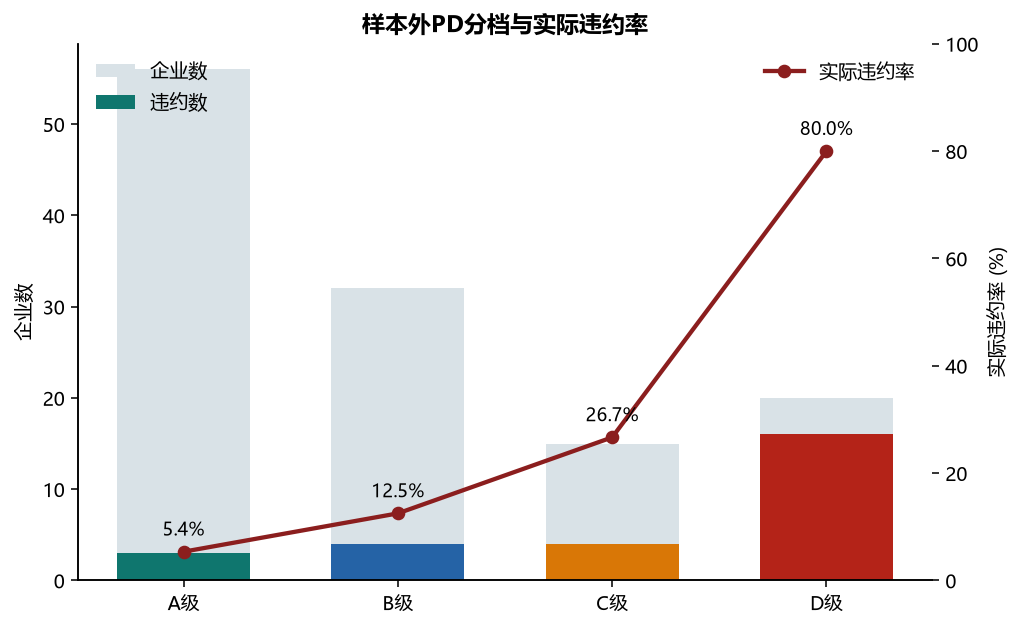
\includegraphics[width=\textwidth]{fig_default_rate.png}
\caption{各PD档实际违约率}
\end{subfigure}\hfill
\begin{subfigure}{0.49\textwidth}
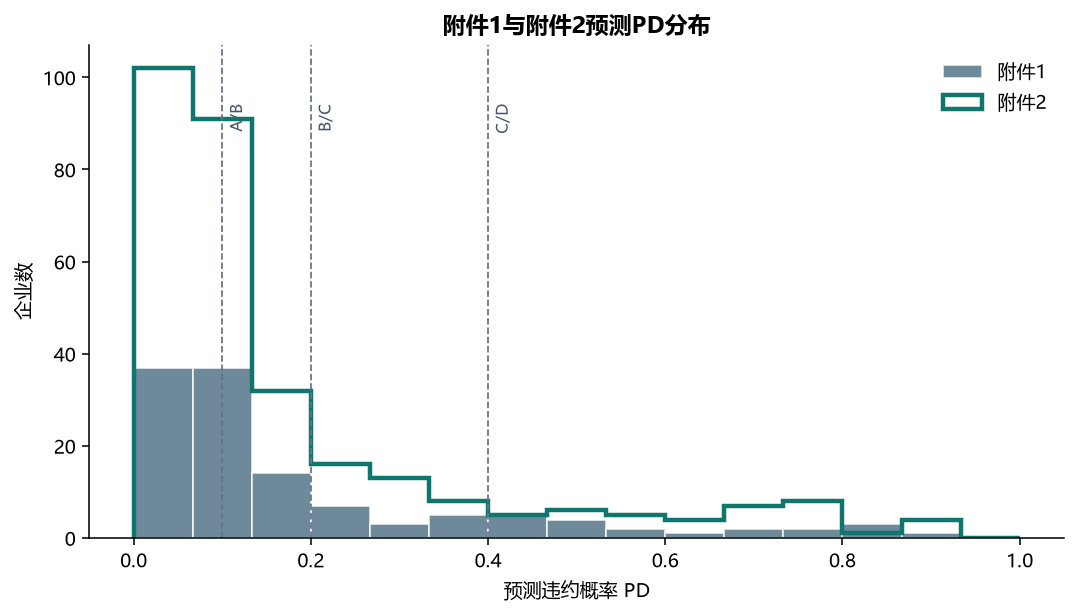
\includegraphics[width=\textwidth]{fig_pd_distribution.png}
\caption{两组企业PD分布}
\end{subfigure}
\caption{PD模型的分档验证与迁移结果}
\end{figure}

\begin{decisionbox}{验证结果意味着什么}
ROC-AUC为\ModelAUC，说明模型能较好地区分风险顺序；D档20家企业中有16家实际违约，实际违约率80.0\%，高风险得到集中识别。A、B、C、D档的实际违约率依次上升，固定阈值具有业务解释力。但附件1只有123家企业，单个档位样本仍少，因此这些概率适合用于组合决策，不应被理解为永不变化的精确真值。
\end{decisionbox}

\begin{figure}[H]
\centering
\begin{subfigure}{0.53\textwidth}
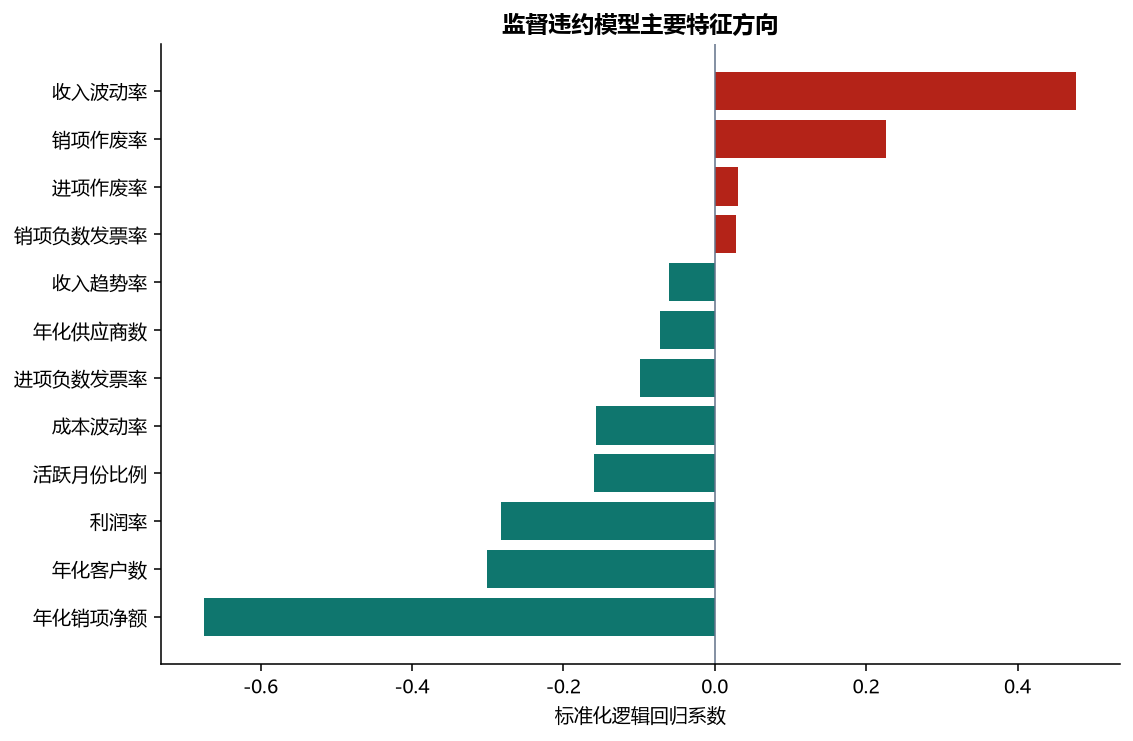
\includegraphics[width=\textwidth]{fig_weights.png}
\caption{标准化特征系数方向}
\end{subfigure}\hfill
\begin{subfigure}{0.43\textwidth}
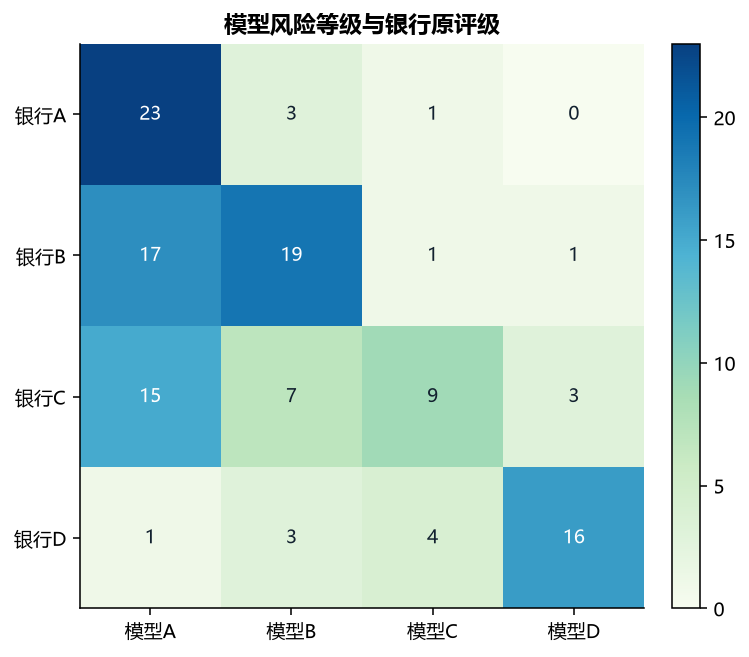
\includegraphics[width=\textwidth]{fig_crosstab.png}
\caption{模型等级与银行原评级}
\end{subfigure}
\caption{风险模型解释与原评级对照}
\end{figure}

系数为正表示该特征增加时模型PD倾向上升，系数为负表示PD倾向下降。由于特征之间可能相关，单个系数反映“其他特征不变时”的方向，不代表直接因果关系。模型等级与银行原评级不完全相同是正常现象：银行评级包含人工经验，模型等级则只依据发票和历史标签。

\section{固定尺度TOPSIS辅助解释}

\subsection{经营质量分数的作用}

逻辑回归回答“企业会不会违约”，TOPSIS回答“企业在经营规模、盈利、稳定和票据行为上离理想状态有多近”。本文使用14项经营质量指标，其中规模、盈利、活跃度和趋势为效益型，波动、断档、作废和负数金额率为成本型\cite{hwang1981}。

对附件1第$j$项指标确定1\%和99\%截尾点并作0至1归一化；附件2沿用附件1的同一边界，超出范围时截到$[0,1]$。正负理想点和权重也只在附件1确定，避免待评价企业改变评分尺子。

设归一化加权向量为$\boldsymbol v_i$，正、负理想点为$\boldsymbol v^+$和$\boldsymbol v^-$，则
\begin{equation}
D_i^+=\|\boldsymbol v_i-\boldsymbol v^+\|_2,
\quad D_i^-=\|\boldsymbol v_i-\boldsymbol v^-\|_2,
\quad S_i=\frac{D_i^-}{D_i^++D_i^-}.
\end{equation}

\begin{intuitionbox}{为什么附件2不能重新归一化}
假设附件1中最高年收入是1000万元，某企业收入500万元，对应相对水平约0.5。如果附件2最高收入只有600万元，并在附件2内重新缩放，同样500万元会变成接近0.83。评分变化来自参照群体而不是企业本身。固定附件1尺度后，同样经营状态得到相同解释。
\end{intuitionbox}

\begin{figure}[H]
\centering
\begin{subfigure}{0.51\textwidth}
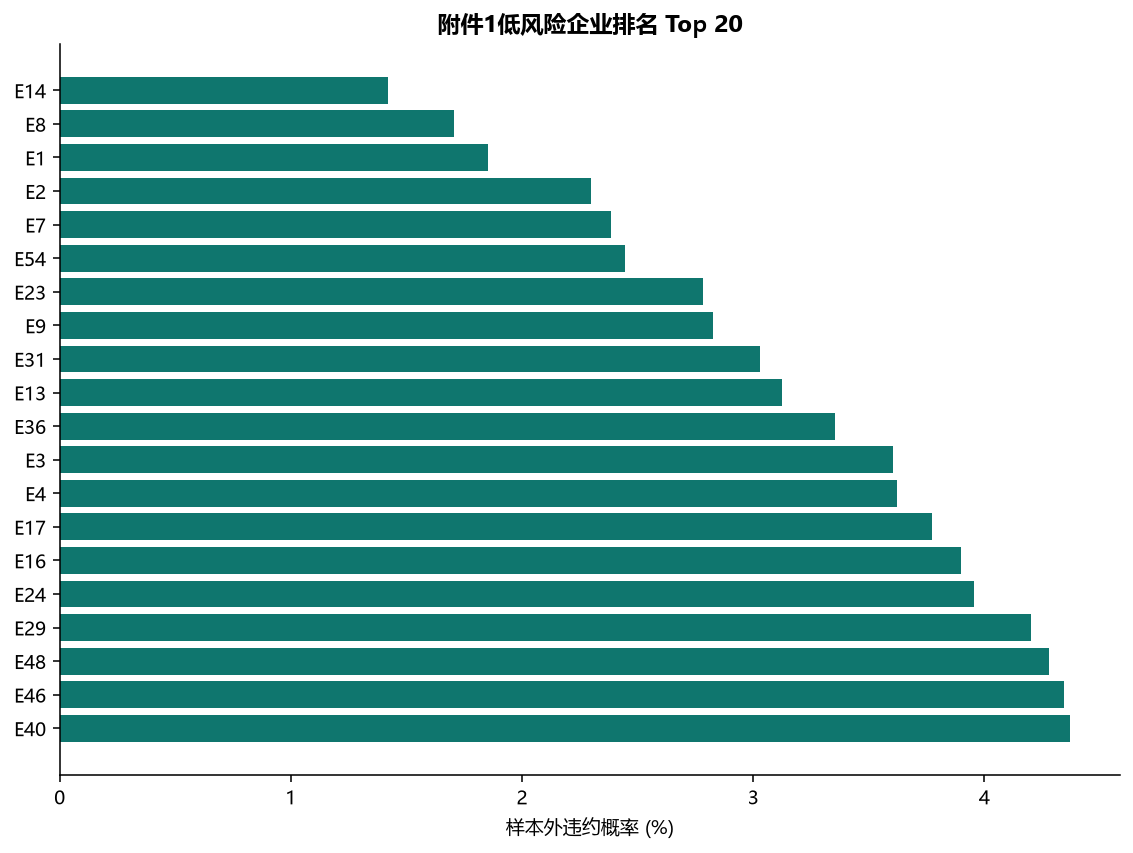
\includegraphics[width=\textwidth]{fig_ranking.png}
\caption{附件1低风险企业}
\end{subfigure}\hfill
\begin{subfigure}{0.45\textwidth}
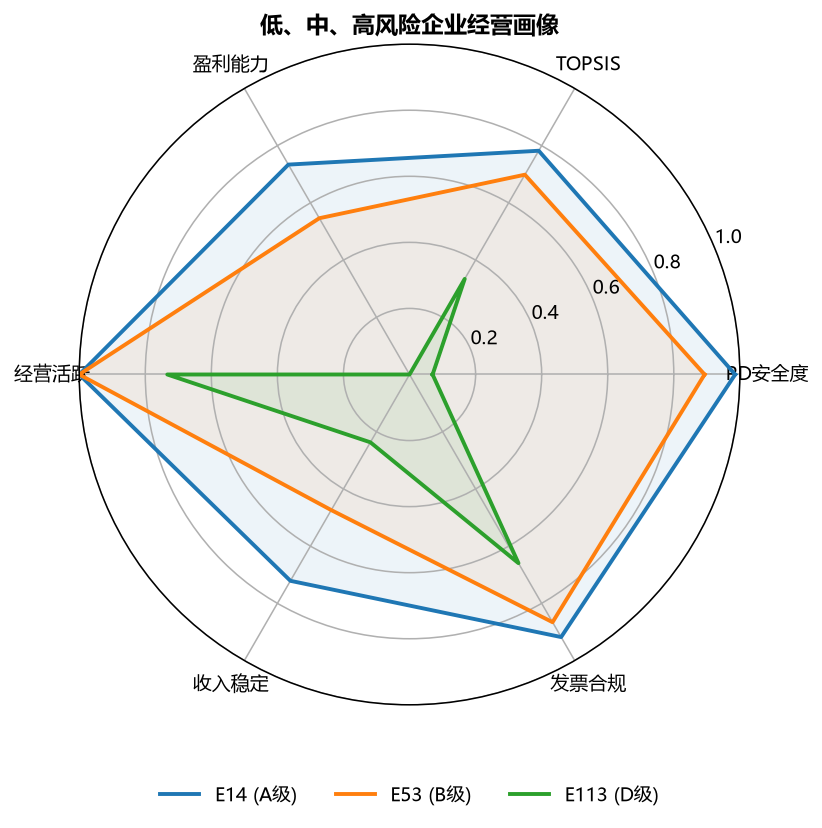
\includegraphics[width=\textwidth]{fig_case_radar.png}
\caption{低、中、高风险企业画像}
\end{subfigure}
\caption{PD风险与TOPSIS经营质量的互补解释}
\end{figure}

TOPSIS得分用于报告排序、个案分析和灵敏度检验，不参与PD档位定义，也不直接决定贷款利率。这样可以避免把主观权重伪装成违约概率，同时保留多指标评价的解释优势。

\section{利率、客户流失与期望收益}

\subsection{为什么利率不能只取最高值}

提高利率会增加每一笔成功贷款的利息，但也可能让客户转向其他银行。特别是低风险企业通常有更多融资渠道，对高利率更敏感。因此利率决策必须同时考虑“每笔赚多少”和“客户是否接受”。

\subsection{保序流失率模型}

附件3的流失率存在少量局部下降点，这可能来自抽样波动。为满足“利率上升时流失率不下降”的经济约束，对A、B、C级分别用PAVA保序回归求解\cite{barlow1972}：
\begin{equation}
\min_{\tilde c_1,\ldots,\tilde c_m}\sum_{k=1}^{m}(c_k-\tilde c_k)^2,
\quad \tilde c_1\le\cdots\le\tilde c_m.
\end{equation}

PAVA会把违反顺序的相邻点合并为加权平均，直到整条曲线非降。任意候选利率的流失率通过分段线性插值得到；D级不进入定价，因为其被禁贷。

\begin{figure}[H]
\centering
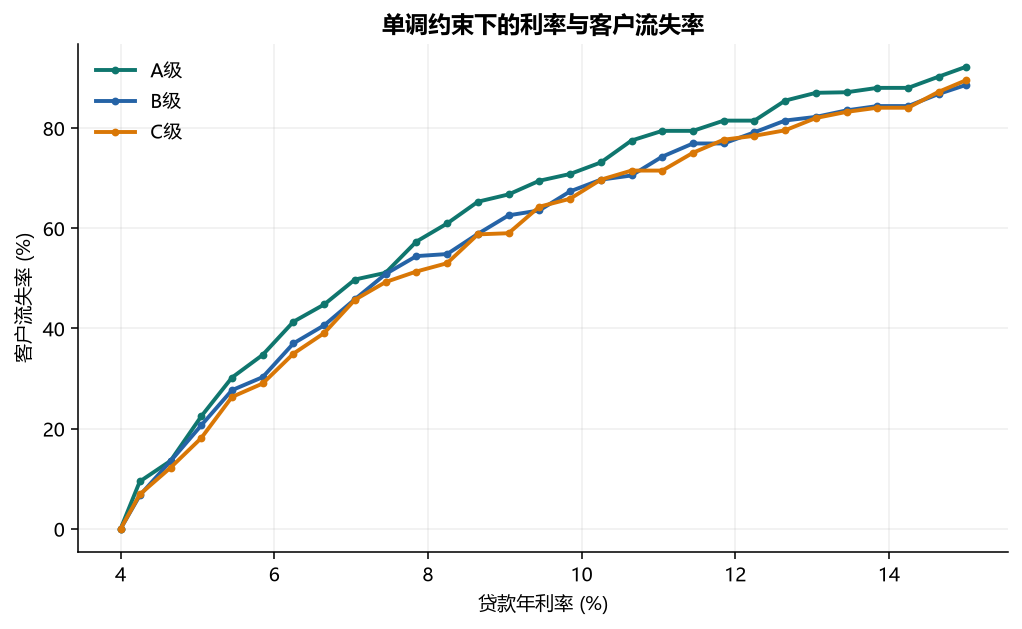
\includegraphics[width=0.77\textwidth]{fig_rate_churn.png}
\caption{单调约束下的利率与客户流失率曲线}
\end{figure}

\subsection{单位额度期望收益}

设企业$i$的PD为$p_i$，利率为$r$，客户留存率为$q_i(r)=1-c_i(r)$，违约损失率为$L$，资金成本率为$c_f$。每1万元名义授信的期望净收益为
\begin{equation}
u_i(r)=q_i(r)\left[(1-p_i)r-p_iL-c_f\right].
\end{equation}

括号内三项分别是未违约利息、违约损失和资金成本；最外层$q_i(r)$表示只有客户留存时才会实际发生放款。对附件3出现过的利率逐点计算$u_i(r)$，选择最大值对应的利率，避免对观测区间之外进行不可靠外推。

\begin{intuitionbox}{100万元贷款的收益怎么算}
假设某企业PD为8\%，利率10\%，流失率20\%，则留存率为80\%。取LGD为60\%、资金成本为2.5\%，每1万元的期望净收益为
\[
0.8\times[(1-0.08)\times0.10-0.08\times0.60-0.025]=0.0152\text{万元}.
\]
如果名义授信100万元，期望净收益约1.52万元。把利率提高后，括号中的利息会增加，但留存率可能下降，净收益不一定提高。
\end{intuitionbox}

\section{混合整数额度优化}

\subsection{从单户收益到银行组合}

即使知道每家企业的最佳利率和单位收益，也不能逐家独立决定额度，因为所有企业共同占用有限预算。令$x_i$为授信额度，$z_i\in\{0,1\}$表示是否授信，优化模型为
\begin{align}
\max_{x,z}\quad &\sum_i u_i^*x_i,\\
\text{s.t.}\quad &\sum_i x_i=B,\\
&10z_i\le x_i\le100z_i,\\
&x_i=0,\quad i\in\{\text{原始D级或预测D级}\}.
\end{align}

第一条约束要求预算精确使用；第二条把“0或10至100万元”转成线性约束；第三条执行D级禁贷。这是一个混合整数线性规划，连续变量$x_i$决定额度，二元变量$z_i$决定是否入选，由SciPy的MILP求解器求全局最优可行解。

\begin{intuitionbox}{用4家企业理解额度分配}
假设4家企业的单位收益依次为2.0\%、1.5\%、0.8\%、$-0.2$\%，预算150万元，单户上限100万元。若没有其他约束，模型会先给第一家100万元，再给第二家50万元，而不会为了“平均”把37.5万元分给每家。真实模型同理：额度首先流向单位收益更高的合格企业。
\end{intuitionbox}

当前目标函数对$x_i$是线性的，且题目只给出统一单户上限，因此最优解通常把入选企业推到100万元上限。若银行希望更加分散，应增加企业申请额度、行业集中度或边际收益递减约束，而不应在求解后随意手工均摊。

\subsection{三问策略结果}

\begin{table}[H]
\centering
\caption{三问信贷策略摘要}
\begin{tabular}{lrrrr}
\toprule
方案 & 放贷企业数 & 额度合计/万元 & 平均利率 & 期望净收益/万元\\
\midrule
问题1 & \PoneLoanCount & \PoneAmount & \PoneAverageRate\% & \PoneNetProfit\\
问题2 & \PtwoLoanCount & \PtwoAmount & \PtwoAverageRate\% & \PtwoNetProfit\\
问题3 & \PthreeLoanCount & \PthreeAmount & \PthreeAverageRate\% & \PthreeNetProfit\\
\bottomrule
\end{tabular}
\end{table}

\begin{figure}[H]
\centering
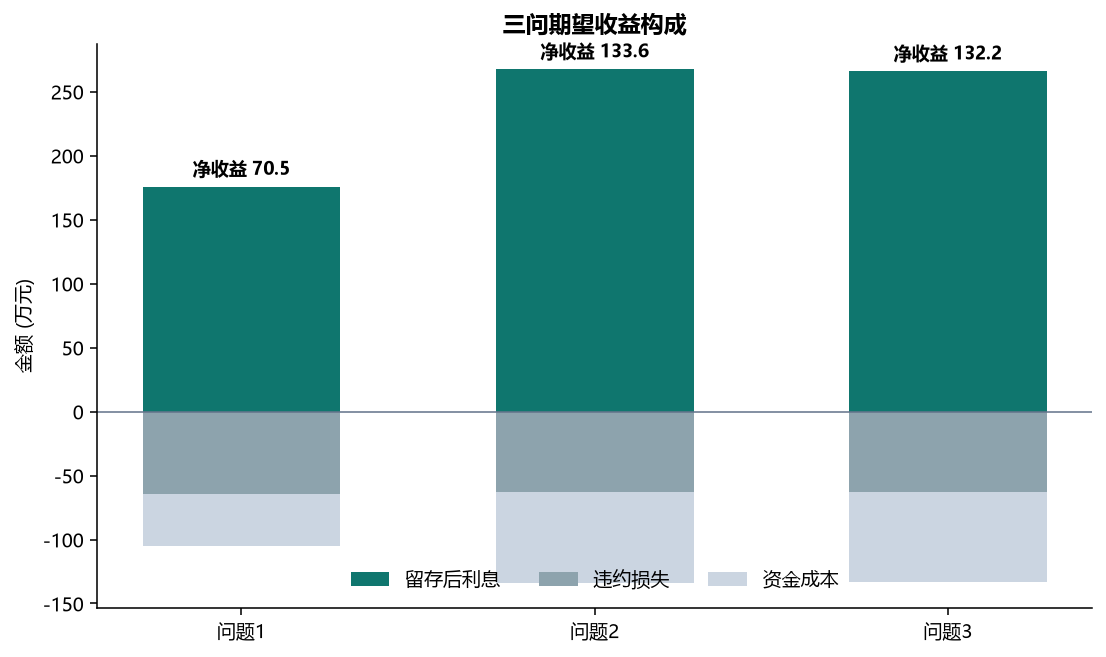
\includegraphics[width=0.82\textwidth]{fig_profit_breakdown.png}
\caption{三问留存后利息、违约损失、资金成本和净收益}
\end{figure}

\begin{decisionbox}{三问结果如何使用}
问题1在8000万元假设预算下向\PoneLoanCount 家企业放贷，问题2在1亿元预算下向\PtwoLoanCount 家企业放贷。原始D级获贷企业数为\OriginalDLoanCount，说明准入规则得到严格执行。净收益是模型期望值而不是保证利润，其意义是用于比较策略和资源配置，不是承诺银行一定获得相同金额。
\end{decisionbox}

\section{疫情冲击下的重新决策}

\subsection{行业分类和冲击系数}

根据企业名称中的行业关键词，把企业划分为严重负面、中度负面、正面或轻影响、其他和未知五类。对于仅有“个体经营E编号”而没有行业语义的企业，标记为未知，不强行猜测行业。严重负面、中度负面和正面或轻影响的赔率系数分别为1.30、1.15和0.90，其他与未知取1.00。

这些系数是可配置压力情景，不是由当前附件估计出的疫情因果效应。若银行获得正式行业代码和疫情期间违约数据，应重新估计行业冲击。

\subsection{为什么冲击作用于赔率}

概率不能无限放大，直接计算$k_ip_i$在高PD时可能超过1。赔率定义为$p/(1-p)$，取正值且没有1的上界，因此令
\begin{equation}
\operatorname{odds}(p_i')=k_i\operatorname{odds}(p_i),
\qquad
p_i'=\frac{k_ip_i}{1-p_i+k_ip_i}.
\end{equation}

\begin{intuitionbox}{赔率调整示例}
若企业原PD为20\%，原赔率为$0.20/0.80=0.25$。严重负面冲击系数1.30使赔率变为0.325，对应新PD为$0.325/(1+0.325)\approx24.5\%$。新概率始终位于0和1之间，而且对原本高风险企业不会产生越界值。
\end{intuitionbox}

调整PD后重新划分等级，再重新选择利率并运行MILP。这样受冲击企业不仅额度可能下降，利率、准入状态和组合中的相对位置也会同步变化。最终共有\EmergencyChanges 家企业跨越风险等级阈值。

\begin{figure}[H]
\centering
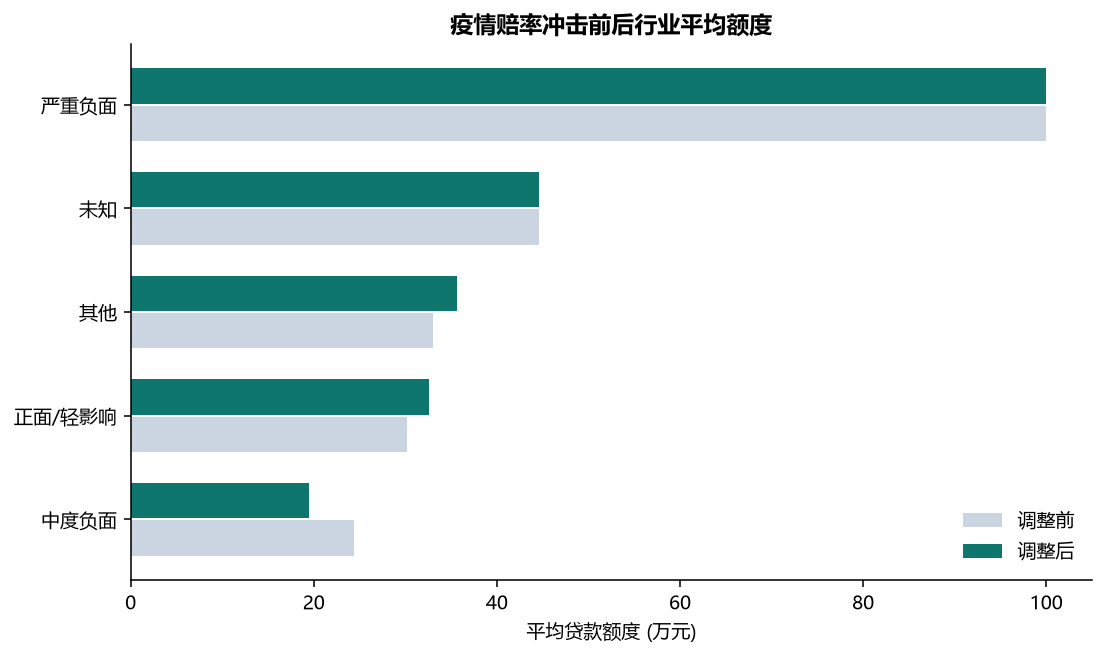
\includegraphics[width=0.82\textwidth]{fig_covid.png}
\caption{疫情赔率冲击前后各行业类别的平均授信额度}
\end{figure}

\begin{decisionbox}{压力测试而不是精确预测}
行业关键词来自脱敏名称，部分企业无法可靠识别。问题3的价值是展示“冲击发生后如何重新决策”的机制，而不是宣称已经准确预测疫情影响。正式应用中应把关键词分类替换为标准行业代码，并用多个冲击系数形成轻度、中度和重度情景。
\end{decisionbox}

\section{灵敏度与稳健性分析}

\subsection{真实权重扰动}

对TOPSIS基准权重进行100次独立扰动，每个权重乘以$U(0.8,1.2)$后重新归一化。每次都从原始特征重新计算TOPSIS得分和完整排名，再与基准排名计算Spearman和Kendall相关系数，而不是围绕某个预设均值随机生成相关系数。

Spearman均值为\SensitivityMean，最小值为\SensitivityMin；Kendall均值为\SensitivityKendall。另逐一移除指标并重新计算，影响最大的指标为“\SensitivityIndicator”，移除后的Spearman相关系数为\SensitivityRemoval。

\begin{figure}[H]
\centering
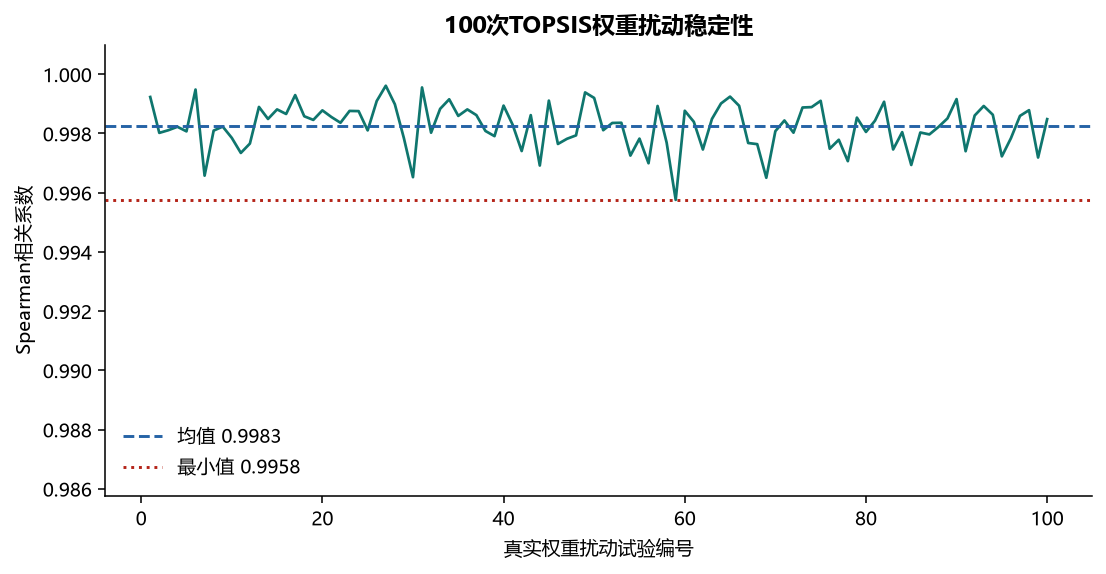
\includegraphics[width=0.82\textwidth]{fig_sensitivity.png}
\caption{100次TOPSIS权重扰动的真实排名相关系数}
\end{figure}

\begin{intuitionbox}{相关系数接近1表示什么}
Spearman相关系数比较两次排名的先后顺序。接近1表示权重稍微变化时，大多数企业仍处于相近位置。它说明TOPSIS解释排名对小幅权重误差较稳定，但不代表PD模型、LGD或资金成本也已经完成同样的敏感性检验。
\end{intuitionbox}

\section{模型评价、局限与扩展}

\subsection{模型优点}

\begin{enumerate}
\item 风险主模型直接学习违约标签，且所有性能指标来自嵌套样本外预测；
\item 发票净额保留负数经济含义，连续月历显式记录经营断档；
\item 附件2不重复拟合缩放尺度，PD和TOPSIS解释具有统一参照；
\item 流失率满足经济意义上的单调性，利率同时考虑收入和客户接受行为；
\item 额度优化严格执行预算、单户上下限和D级禁贷，并导出收益拆分；
\item 图表、Excel、网页和论文数字由同一次运行生成，降低手工抄录错误。
\end{enumerate}

\subsection{主要局限}

第一，附件1只有123家企业，无法充分覆盖所有行业和经营状态。当前样本外验证比训练内评价可靠，但仍不能替代跨年份、跨地区的外部验证。

第二，LGD为60\%、资金成本为2.5\%、问题1预算为8000万元，这些是显式情景假设，不是附件直接给出的事实。银行应按真实参数重跑，并比较参数变化对企业入选名单和收益的影响。

第三，模型假定PD在利率选择阶段不随利率变化。现实中高利率可能增加企业偿债压力，使PD进一步上升。若有历史定价和贷后表现数据，可建立利率、PD和流失率的联合模型。

第四，疫情行业识别依赖脱敏名称，信息不足的企业只能标记为未知。冲击结果适合用于压力测试，不适合作为真实行业风险的精确估计。

第五，当前线性目标会把入选企业推向单户上限，尚未包含企业真实资金需求、行业集中度、资本占用和组合尾部风险。

\subsection{扩展方向}

获得新增样本后，可按时间滚动进行外部验证和概率再校准；获得回收数据后，可把LGD从常数扩展为企业层面模型；获得申请额度后，可把单户上限改为100万元与实际需求的较小值；需要控制组合风险时，可增加行业额度上限、期望损失上限或CVaR约束。上述扩展均不改变“PD估计、定价、组合优化”的主体结构。

\section{结论}

本文从发票净额和经营连续性出发，建立带正则、类别平衡和先验校正的监督PD模型，并用重复嵌套交叉验证获得严格样本外结果。模型ROC-AUC达到\ModelAUC，A至D档实际违约率依次上升，能够集中识别高风险企业。TOPSIS被限定为经营质量辅助解释工具，从而避免综合评分与违约概率的概念混淆。

进一步地，本文用保序回归建立利率与客户流失率的单调关系，把留存后利息、违约损失和资金成本合并为单位额度期望收益，再通过混合整数规划满足预算、准入和单户额度约束。三问预算均被精确满足，原始D级获贷企业数为\OriginalDLoanCount。疫情情景通过赔率调整后触发完整的重新评级、定价和额度优化。

模型的核心不是给企业生成一个孤立分数，而是建立从数据口径、风险概率、客户行为到银行资源配置的一致链条。每一步都能解释、复算和替换参数，这使模型既适合数学建模竞赛展示，也为后续接入真实银行数据保留了扩展空间。

\begin{thebibliography}{9}
\small
\setlength{\itemsep}{0pt}
\setlength{\parskip}{0pt}
\bibitem{hosmer2013} Hosmer D W, Lemeshow S, Sturdivant R X. Applied Logistic Regression. Wiley, 2013.
\bibitem{hastie2009} Hastie T, Tibshirani R, Friedman J. The Elements of Statistical Learning. Springer, 2009.
\bibitem{hwang1981} Hwang C L, Yoon K. Multiple Attribute Decision Making: Methods and Applications. Springer, 1981.
\bibitem{barlow1972} Barlow R E, Bartholomew D J, Bremner J M, Brunk H D. Statistical Inference under Order Restrictions. Wiley, 1972.
\end{thebibliography}

\end{document}
